\documentclass[aspectratio=169]{beamer}

\usetheme{NRLpresentationGWU}
\usepackage{NRLcolors}

%\titlegraphic{\includegraphics[width=0.9\textwidth]{$HOME/Documents/TAVEX/gmt/TAVEX-overview-3}}% optional

\setbeamerfont{footnote}{size=\tiny}
%\beamertemplatenavigationsymbolsempty


\usepackage[style=authortitle-comp,maxnames=1]{biblatex} % PGR: backend=biber???
%\addbibresource{../References/PhD_refs.bib}
\addbibresource{references.bib}

\usepackage{graphicx}
\graphicspath{{../../Figures/}}

\usepackage{amsmath,amssymb,amsfonts}
\usepackage{upgreek}
\usepackage[retainorgcmds]{IEEEtrantools}

%\usepackage{hyperref}
%\usepackage[capitalize]{cleveref}

\usepackage{mathtools}
\usepackage{relsize}

\usepackage{bm}
\usepackage{hhline}
\usepackage{xcolor}


\setlength{\fboxsep}{3pt}
\setlength{\fboxrule}{2pt}


\usepackage{mathfont_shortcuts}
\usepackage{PhDmath}


\newcommand{\indep}{\perp \!\!\! \perp}
%\DeclareMathOperator*{\indep}{\perp \!\!\! \perp}
\newcommand\independent{\protect\mathpalette{\protect\independenT}{\perp}}
\def\independenT#1#2{\mathrel{\rlap{$#1#2$}\mkern2mu{#1#2}}}




\title{Bayesian Learning for Regression using Dirichlet Prior Distributions of Varying Localization}
%\subtitle{Work Supported by the U.S. Office of Naval Research}% optional

\author[Rademacher \& Doroslova\v{c}ki]{Paul Rademacher\inst{1} \and Milo\v{s} Doroslova\v{c}ki\inst{2}}
\institute[NRL,~GWU] 
{
  \inst{1}
  U.S. Naval Research Laboratory\\Radar Division
  \and
  \inst{2}
  The George Washington University\\Department of Electrical and Computer Engineering
}


\date{July 11, 2021}


%\NRLcredit{Work Supported by the U.S. Office of Naval Research}% optional
%\NRLmark{FOR OFFICIAL USE ONLY}% optional
%\NRLpatents{Example Patents\\7,749,438 and 7,754,145}% optional

\NRLdist{DISTRIBUTION A. Approved for public release: distribution unlimited.}
%\NRLfoot{DISTRIBUTION A. Approved for public release: distribution unlimited.}


\begin{document}


\begin{frame}
\titlepage
\end{frame}


\section{Introduction} 

\begin{frame}
\frametitle{Bayesian Learning}
%\frametitle{Introduction}
%\framesubtitle{Part I}

Bayesian approaches to statistical learning attempt to make better decisions by exploiting \alert{prior knowledge} regarding the data-generating distribution:

\vspace{1em}

\begin{columns}[T]

\begin{column}{.5\linewidth}

\centering
\large \textbf{\underline{Informative}} \normalsize
\vspace{0.5em}
\begin{itemize}
\item If the prior is localized around the true data-generating model, low-risk decisions can be made even with limited training data
\item Priors that assign low weighting to the true model may not be able to realize satisfactory performance 
\end{itemize}


\end{column}

\vrule

\begin{column}{.5\linewidth}

\centering
\large \textbf{\underline{Non-Informative}} \normalsize
\vspace{0.5em}
\begin{itemize}
\item Learners designed with minimally localized priors respond strongly to training data, avoiding the drawbacks of misinformed prior knowledge
\item If the data volume is limited, high variance ``overfit'' solutions can occur
%\item Learners designed with approximately uniform priors will not perform as well as those made with well-selected informative priors
%\item Avoid high risk inherent to learners made by mismatched informative priors
\end{itemize}



\end{column}

\end{columns}

\end{frame}




\begin{frame}
\frametitle{The Dirichlet Prior}
%\frametitle{Introduction}
%\framesubtitle{Part II}

Dirichlet prior distributions have a number of desirable properties:
\begin{itemize}
%\item Often, priors are termed non-informative as long as they are approximately uniform over their \underline{limited support}. For example, a parametric regression function might use a high covariance Gaussian vector prior to characterize a subset of probability distributions
\vspace{0.5em}
\item \alert{Full support} over the space of data-generating distributions, guaranteeing \emph{consistent estimation} of the true data model
\vspace{0.5em}
\item They are \alert{conjugate priors} for independent, identically distributed observations \footfullcite{ferguson}, leading to \emph{closed-form} posterior distributions
\vspace{0.5em}
\item \alert{Flexible parameterization} enabling \emph{both} maximally and minimally informative priors and thus a wide range of learning solutions
\end{itemize}

\end{frame}



\section{Data Model and Regression Objective}


\begin{frame}
\frametitle{Data Representation}

\begin{description}
\item[Observable random variable:] $\xrm \in \Xcal \subset \Rbb$
\item[Unobservable random variable:] $\yrm \in \Ycal \subset \Rbb$
\item[Observable training data:] $\Drm \in \Dcal = \{\Ycal \times \Xcal\}^N$
\end{description}

\vspace{0.5em}

Independently, identically distributed according to an \alert{unknown} probability mass function (PMF) 
\begin{equation*}
\uptheta \in \Theta = \left\{ \theta \in {\Rbb_{\geq 0}}^{\Ycal \times \Xcal}: \sum_{y \in \Ycal} \sum_{x \in \Xcal} \theta(y,x) = 1 \right\} \ ,
\end{equation*}
such that $\Prm_{\yrm,\xrm | \uptheta}(y,x | \theta) = \Prm_{\Drm_n | \uptheta}(y,x | \theta) = \theta(y,x)$.

\hrulefill

\vspace{0.5em}
\textit{Alternate Notation}: $\uptheta \Leftrightarrow \big( \upthetam,\upthetac \big)$
\begin{itemize}
\item Marginal model $\upthetam \equiv \sum_{y \in \Ycal} \uptheta(y,\cdot) = \Prm_{\xrm | \uptheta} \equiv \Prm_{\xrm | \upthetam}$
\item Conditional models $\upthetac(x) \equiv \uptheta(\cdot,x) / \upthetam(x) = \Prm_{\yrm | \xrm,\uptheta} \equiv \Prm_{\yrm | \xrm,\upthetac}$ 
\end{itemize}

\end{frame}




\begin{frame}
\frametitle{Sufficient Statistic}
\framesubtitle{Transform}

\begin{columns}[c]

\begin{column}{.5\linewidth}

Using the i.i.d. assumption,
\begin{IEEEeqnarray}{C}
\Prm_{\Drm | \uptheta}\big( D | \theta \big) = \left( \prod_{y \in \Ycal} \prod_{x \in \Xcal} \theta(y,x)^{\Psi(y,x;D)} \right)^N \nonumber 
\end{IEEEeqnarray}
where data are represented using $\Psi : \Dcal \mapsto \Uppsi \subset \Theta$, defined as
\begin{equation*}
\Psi(y,x;D) = N^{-1} \sum_{n=1}^N \delta \big[ (y,x),D_n \big] \;.
\end{equation*}
%and the range is
%\begin{equation*}
%\Uppsi = \left\{ \frac{n}{N} \in {\Zbb_{\geq 0}}^{\Ycal \times \Xcal}: \sum_{y \in \Ycal} \sum_{x \in \Xcal} n(y,x) = N \right\}
%\end{equation*}

\end{column}

\vrule
\hspace{0.5ex}
\begin{column}{.5\linewidth}

\begin{itemize}
\item Empirical distribution $\Psi(\Drm)$ is a \alert{sufficient statistic}\footnotemark ~for the model $\uptheta$
\vspace{0.5em}
\item Efficient: $|\Uppsi| = \binom{N+|\Ycal||\Xcal|-1}{|\Ycal||\Xcal|-1} \leq |\Dcal|$
\vspace{1.5em}
\item [$\Rightarrow$] \textbf{Represent data using new random process $\uppsi \equiv \Psi(\Drm) \in \Uppsi$}

%\vspace{0.5em}
%\item \textit{Alternate Notation}: $\uppsi \Leftrightarrow \big( \uppsim,\uppsic \big)$
%\begin{itemize}
%\item Marginal $\uppsim \equiv \sum_{y \in \Ycal} \uppsi(y,\cdot)$
%\item Conditional $\uppsic(\xrm) \equiv \uppsi(\cdot,\xrm) / \uppsim(x)$
%\end{itemize}
\end{itemize}

\end{column}

\end{columns}

\footcitetext{bernardo}
%\footcitetext{feller}

\end{frame}



\begin{frame}
\frametitle{Sufficient Statistic}
\framesubtitle{Distribution}

\begin{itemize}
\item Conditioned on the true model, the data statistic is an ``Empirical'' random process $\uppsi | \uptheta \sim \Emp(N,\uptheta)$
\begin{itemize}
\item Equivalent to a normalized multinomial random process \footfullcite{minka-multi}
\end{itemize}
\item As $N \to \infty$, the random process converges to $\uppsi | \uptheta \inprob \uptheta$
\begin{itemize}
\item [$\Rightarrow$] Use enables \alert{consistent} estimation of model
\end{itemize}

\end{itemize}



\hrulefill
\vspace{.5em}

\begin{columns}[c]

\begin{column}{.5\linewidth}
\textit{Alternate Notation}: $\uppsi \Leftrightarrow \big( \uppsim,\uppsic \big)$
\begin{itemize}
\item Marginal $\uppsim \equiv \sum_{y \in \Ycal} \uppsi(y,\cdot)$
\item Conditional $\uppsic(x) \equiv \uppsi(\cdot,x) / \uppsim(x)$
\end{itemize}
\end{column}

\begin{column}{.5\linewidth}
By the aggregation property \footnotemark,
\begin{itemize}
\item $\uppsim | \upthetam \sim \Emp(N,\upthetam)$
\item $\uppsic(x) | \uppsim(x),\upthetac(x) \sim \Emp\big( N \uppsim(x),\upthetac(x) \big)$ are mutually \alert{independent}
\end{itemize}
\end{column}

\end{columns}

\footcitetext{johnson}

\end{frame}



\begin{frame}
\frametitle{Objective}

\begin{itemize}
\item Design a regression function $f: \Uppsi \mapsto \Rbb^{\Xcal}$ to minimize the expected squared-error with respect to $\uptheta$:
\begin{IEEEeqnarray}{rCl} \label{eq:risk_cond_SE}
\Rcal_{\Theta}(f ; \uptheta) = \Erm_{\yrm,\xrm,\uppsi | \uptheta} \Big[ \big( f(\xrm;\uppsi)-\yrm \big)^2 \Big] & \equiv & \underbrace{\Erm_{\xrm | \upthetam} \left[ \Sigma_{\yrm | \xrm,\upthetac} \right]}_{\mathlarger{\Rcal_{\Theta}^*(\uptheta)}} + \underbrace{\Erm_{\xrm,\uppsi | \uptheta} \Big[ \big( f(\xrm;\uppsi) - \mu_{\yrm | \xrm,\upthetac} \big)^2 \Big]}_{\mathlarger{\Rcal_{\Theta, \mathrm{ex}}(f ; \uptheta)}} \nonumber
\end{IEEEeqnarray}

\item Clairvoyant \footfullcite{kay-det} regressor $f_{\Theta}(\xrm;\upthetac) = \mu_{\yrm | \xrm,\upthetac}$ achieves \emph{irreducible} squared-error $\Rcal_{\Theta}^*(\uptheta)$

\item Excess squared-error can be decomposed into \alert{bias} and \alert{variance} terms:
\begin{IEEEeqnarray}{rCl} \label{eq:risk_cond_ex_SE}
\Rcal_{\Theta, \mathrm{ex}}(f ; \uptheta) & \equiv & \Erm_{\xrm | \upthetam} \left[ \Big( \Erm_{\uppsi | \uptheta}\big[ f(\xrm;\uppsi) \big] - f_{\Theta}(\xrm;\upthetac) \Big)^2 + \Crm_{\uppsi | \uptheta}\big[ f(\xrm;\uppsi) \big] \right] \nonumber 
\end{IEEEeqnarray}

\end{itemize}

\end{frame}




\begin{frame}
\frametitle{Bayesian Inference}

\textbf{Model unknown. Select prior $\prm_\uptheta$ and formulate Bayesian risk:}
\begin{IEEEeqnarray}{rCl} \label{eq:risk}
\Rcal(f) & = & \Erm_{\uptheta}\big[ \Rcal_{\Theta}(f ; \uptheta) \big] = \Erm_{\yrm,\xrm,\uppsi} \Big[ \big( f(\xrm;\uppsi)-\yrm \big)^2 \Big] \nonumber
\end{IEEEeqnarray}

%\large
%\begin{equation*} 
%\Downarrow \quad \Downarrow \quad \textbf{\textit{Model Unknown. Select Prior }} \bm{\mathrm{p}_\uptheta} \quad \Downarrow \quad \Downarrow 
%\end{equation*}
%\normalsize
%\begin{IEEEeqnarray}{rCl} \label{eq:risk}
%\Rcal(f) & = & \Erm_{\uptheta}\big[ \Rcal_{\Theta}(f ; \uptheta) \big] = \Erm_{\yrm,\xrm,\uppsi} \Big[ \big( f(\xrm;\uppsi)-\yrm \big)^2 \Big] \nonumber
%\end{IEEEeqnarray}

\vspace{-3em}
\huge
\begin{equation*} 
\Downarrow \quad \Downarrow \quad \Downarrow \quad \Downarrow 
\end{equation*}
\normalsize

\textbf{Bayes optimal regressor:}
\begin{IEEEeqnarray}{rCl} \label{eq:f_opt_xD}
f^*(\xrm;\uppsi) & = & \argmin_{y' \in \Rbb} \Erm_{\yrm | \xrm,\uppsi}\big[ (y'-\yrm)^2 \big] = \textcolor[rgb]{1,0,0}{\mu_{\yrm | \xrm,\uppsi}} \nonumber
\end{IEEEeqnarray}

\vspace{-.5em}
\begin{itemize}
\item[$*$] Observe that $\Prm_{\yrm | \xrm,\uppsi} = \Erm_{\uptheta | \xrm,\uppsi}\big[ \Prm_{\yrm | \xrm,\uptheta} \big] \equiv \mu_{\upthetac(\xrm) | \xrm,\uppsi}$
\end{itemize}

\vspace{1em}

\centering
\fcolorbox{NRL_blue}{NRL_blue}{\color{white}
\parbox{37em}{
\centering
\large
\textbf{Bayesian distribution is the posterior mean \footfullcite{murphy} of the predictive model $\upthetac$}
}
}

\vspace{1em}

%Note: the Bayesian distribution $\Prm_{\yrm | \xrm,\uppsi} = \Erm_{\uptheta | \xrm,\uppsi}\big[ \Prm_{\yrm | \xrm,\uptheta} \big] \equiv \mu_{\upthetac(\xrm) | \xrm,\uppsi}$ is the posterior mean \footfullcite{murphy} of the true predictive model $\upthetac$

%\begin{itemize}
%\item Bayes optimal regressor = $\mu_{\yrm | \xrm,\uppsi}$
%\begin{itemize}
%\item[$*$] Note: Bayesian predictive distribution is the expectation of the true predictive distribution, $\Prm_{\yrm | \xrm,\uppsi} = \Erm_{\uptheta | \xrm,\uppsi}\big[ \Prm_{\yrm | \xrm,\uptheta} \big]$
%\end{itemize}
%\end{itemize}

\end{frame}









\section{Distributions: Prior to Predictive}


\begin{frame}
\frametitle{Dirichlet Prior}

\begin{columns}[c]

\begin{column}{.8\linewidth}

The probability density function of the model $\uptheta \in \Theta$ is Dirichlet:
\begin{IEEEeqnarray*}{L}
\prm_{\uptheta}(\theta) = \Dir(\theta; \alpha_0,\alpha) \equiv \beta(\alpha_0 \alpha)^{-1} \prod_{y \in \Ycal} \prod_{x \in \Xcal} \theta(y,x)^{\alpha_0 \alpha(y,x) - 1}
\end{IEEEeqnarray*}

%\footcitetext{bishop}

\vspace{-1em}
\begin{itemize}
\item Parameter $\alpha_0$ controls localization around mean $\alpha$
\end{itemize}

\vspace{1em}

\textit{Alternate Notation}: 
\begin{itemize}
\item Marginal $\alpham \equiv \sum_{y \in \Ycal} \alpha(y,\cdot)$ 
\item Conditional $\alphac(x) \equiv \alpha(\cdot,x) / \alpham(x)$
\item[$*$] By the aggregation property\footnotemark, $\upthetam \sim \Dir(\alpha_0,\alpham)$ and $\upthetac(x) \sim \Dir\big(\alpha_0 \alpham(x),\alphac(x)\big)$ are mutually \alert{independent}
\end{itemize}


\end{column}


\begin{column}{.2\linewidth}

\begin{figure}
\centering
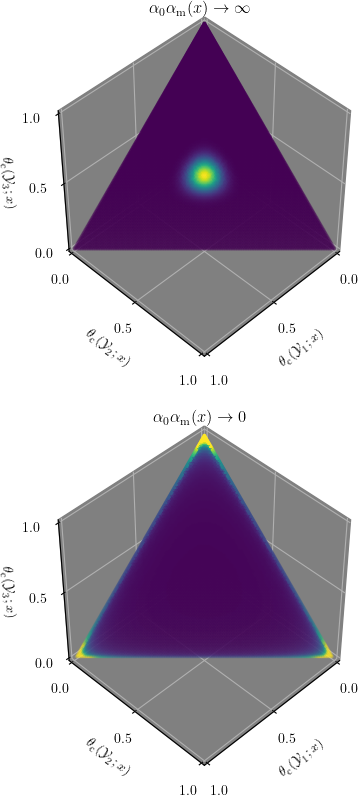
\includegraphics[width=1\linewidth]{SSP_2021/presentation/dir_loc.png}
%\caption{}
\end{figure}

\end{column}

\end{columns}

\vspace{-.75em}
\footcitetext{ferguson}


\end{frame}




\begin{frame}
\frametitle{Predictive Model Posterior}
\framesubtitle{Closed-Form}

Since $\indep_x \upthetac(x)$ and $\upthetac \indep \upthetam$, and since the Empirical process $\upthetac(x) | \uppsim(x),\uppsic(x)$ has exponential form, Dirichlet process $\upthetac(x)$ is conjugate \footfullcite{theodoridis-ML} and thus
%\vspace{-.5em}
\begin{IEEEeqnarray*}{L}
	\upthetac(x) | \uppsim(x),\uppsic(x) \sim \Dir\Big( \alpha_0 \alpham(x) + N \uppsim(x), \mu_{\upthetac(x) | \uppsim(x), \uppsic(x)} \Big) \;,
\end{IEEEeqnarray*}
%\vspace{-.5em}
with mean functions
\begin{IEEEeqnarray*}{rCl} \label{eq:pred_Bayes_psi}
	\mu_{\upthetac(x) | \uppsim(x), \uppsic(x)} & = & \gamma(x; \uppsim) \alphac(x) + \big(1 - \gamma(x; \uppsim)\big) \uppsic(x) \equiv \textcolor[rgb]{1,0,0}{\Prm_{\yrm | \xrm,\uppsi}} \;,
\end{IEEEeqnarray*}
%\begin{IEEEeqnarray*}{rCl} \label{eq:pred_Bayes_psi}
%	\mu_{\upthetac(x) | \uppsim(x), \uppsic(x)} & = & \gamma(x; \uppsim) \underbrace{\alphac(x)}_{\mathclap{= \mu_{\upthetac(\xrm)} = \Prm_{\yrm | \xrm}}} + \big(1 - \gamma(x; \uppsim)\big) \uppsic(x) \equiv \textcolor[rgb]{1,0,0}{\Prm_{\yrm | \xrm,\uppsi}} \;,
%\end{IEEEeqnarray*}
where $\gamma(x; \uppsim) = \Big( 1 + N \uppsim(x) / \big(\alpha_0 \alpham(x)\big) \Big)^{-1} \in (0,1]$.

\vspace{1em}

\centering
\fcolorbox{NRL_blue}{NRL_blue}{\color{white}
\parbox{37em}{
\centering
\large
\textbf{Bayesian predictions mix prior mean $\alphac$ with empirical distribution $\uppsic$}
}
}

\end{frame}



\begin{frame}
\frametitle{Predictive Model Posterior}
\framesubtitle{Trends}

\begin{columns}[c]

\begin{column}{.5\linewidth}

\begin{itemize}
\item As localization $\alpha_0$ increases, $\upthetac(x) | \uppsim(x),\uppsic(x) \inprob  \alphac(\xrm)$ and the prior is emphasized
\vspace{1em}
\item As training volume $N$ increases, $\upthetac(x) | \uppsim(x),\uppsic(x) \inprob \uppsic(x)$ and data is emphasized
\begin{itemize}
\item[$*$] Since $\uppsic | \upthetac \inprob \upthetac$, the true predictive model is \alert{identified}
\end{itemize}
\end{itemize}


\end{column}

\begin{column}{.5\linewidth}

\begin{figure}
\centering
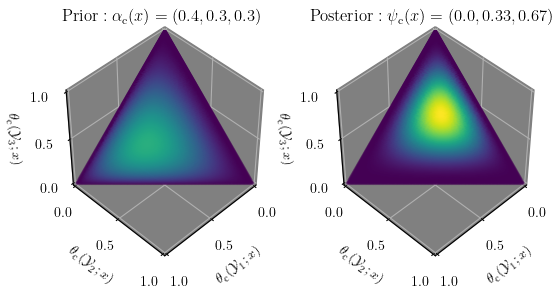
\includegraphics[width=1\linewidth]{SSP_2021/presentation/prior_post_h.png}
%\caption{}
\label{fig:P_theta_post_uni}
\end{figure}

\end{column}

\end{columns}


\vspace{1em}

\centering
\fcolorbox{NRL_blue}{NRL_blue}{\color{white}
\parbox{37em}{
\centering
\large
\textbf{Full support prior ensures consistent estimation of model}
}
}

\end{frame}



\begin{frame}
\frametitle{Bayes Optimal Regressor}

\textbf{Regressor}: $f^*(\xrm;\uppsi) \equiv \gamma(\xrm; \uppsim) \mu_{\yrm | \xrm} + \big(1-\gamma(\xrm; \uppsim)\big) \sum_{y \in \Ycal} \uppsic(y;\xrm) \ y$
\vspace{.5em}
\begin{itemize}
%\item[$*$] $\Prm_{\yrm | \xrm} = \mu_{\upthetac(\xrm)} = \alphac(\xrm)$
\item[$*$] Convexly combines first moment of $\Prm_{\yrm | \xrm} = \mu_{\upthetac(\xrm)} = \alphac(\xrm)$ with empirical mean 
\item[$*$] Inherits trends from posterior distribution, allowing maximal or minimal confidence in the prior
\end{itemize}

\hrulefill
\vspace{1.5em}

\textbf{Excess SE}: $\Rcal_{\Theta, \mathrm{ex}}(f^* ; \uptheta) \equiv \Erm_{\xrm | \upthetam}\Big[ \lambda_{\text{Bias}}(\xrm; \upthetam) \left( \mu_{\yrm | \xrm} - \mu_{\yrm | \xrm,\upthetac} \right)^2 + \lambda_{\text{Var}}(\xrm; \upthetam) \Sigma_{\yrm | \xrm,\upthetac} \Big]$
\begin{itemize}
\item[$*$] \footnotesize $\lambda_{\text{Bias}}(x; \upthetam) = \Erm_{\uppsim | \upthetam}\left[ \gamma(x; \uppsim)^2 \right]$ and $\lambda_{\text{Var}}(x; \upthetam) = \Erm_{\uppsim | \upthetam}\left[ \frac{\big( 1 - \gamma(x; \uppsim) \big)^2}{N \uppsim(x)} \right]$ \normalsize
\end{itemize}

\begin{itemize}
\item \alert{Bias}: proportionate to squared-difference between data-independent regressor $\mu_{\yrm | \xrm}$ and clairvoyant regressor
\item \alert{Variance}: proportionate to the predictive variance, adding to the irreducible risk
\end{itemize}

\end{frame}






\section{Trends and Results}


\begin{frame}
\frametitle{Example}

\begin{columns}[T]

\begin{column}{.5\linewidth}

\textbf{Data Model}:
\begin{itemize}
\item $\Xcal = \Ycal = \{i/127: i = 0, \ldots, 127\}$
%\item $\Xcal$ and $\Ycal$ are 128-point discretizations of $[0,1]$
\item $\thetam = |\Xcal|^{-1}$
%\item $\thetac(y;\xrm) = \DE\big((y, 1-y); 127, 4.164, (\mu_{\yrm | \xrm,\uptheta}, 1-\mu_{\yrm | \xrm,\uptheta})\big)$
%\item $\thetac(y; \xrm) = \Bi\big(127y; 127, \mu_{\yrm | \xrm,\upthetac}\big)$
\item \alert{Clairvoyant}: $\mu_{\yrm | \xrm,\upthetac} = 1 / \big(2 + \sin(2\pi \xrm\big)$
\item $\Sigma_{\yrm | \xrm, \uptheta} = 0.2 \, \mu_{\yrm | \xrm, \uptheta} (1 - \mu_{\yrm | \xrm, \uptheta})$
\begin{itemize}
\item[$\Rightarrow$] $\Rcal_{\Theta}^*(\uptheta) \approx 0.039$
\end{itemize}
\end{itemize}


\end{column}

\begin{column}{.5\linewidth}

\textbf{Learners}:
\begin{itemize}
\item Dirichlet:
\begin{itemize}
\item $\alpham = |\Xcal|^{-1}$ 
%\item $\alphac(y;x) = \DE\big((y, 1-y); 127, 4.164, (0.5, 0.5)\big)$
%\item $\alphac(y; \xrm) = \Bi(127y; 127, \mu_{\yrm | \xrm})$
\item \alert{Prior} $\mu_{\yrm | \xrm} = 0.5$
\end{itemize}

\item Normal\footnotemark:
\begin{itemize}
\item $\yrm | \xrm, \uptheta \sim \Ncal\big([1, \xrm] \uptheta, 0.1 \big)$ 
\item $\uptheta \sim \Ncal\big([0.5, 0], \Sigma_{\uptheta}\big)$
\end{itemize}
\end{itemize}


\end{column}

\end{columns}

\vspace{1em}

\begin{itemize}
\item \emph{Prior confidence} of Dirichlet and Normal learners varied using $\alpha_0$ and $\Sigma_{\uptheta}$
\vspace{.5em}
\item Both learners effect the same \alert{biased} untrained regressor to approximate the non-linear clairvoyant regressor
\end{itemize}


\footcitetext{theodoridis-ML}

\end{frame}


\begin{frame}
\frametitle{Prediction Statistics}

\begin{columns}[c]

\begin{column}{.5\linewidth}

\begin{figure}
	\centering
	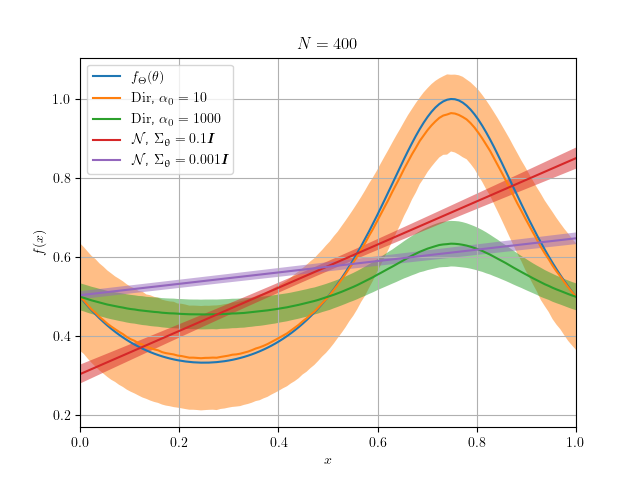
\includegraphics[width=1\linewidth]{Discrete/SE/predict_a0.png}
%	\caption{Predictor mean/variance, comparative}
	\label{fig:Discrete/SE/predict_a0}
\end{figure}

\end{column}

\begin{column}{.5\linewidth}

\begin{figure}
	\centering
	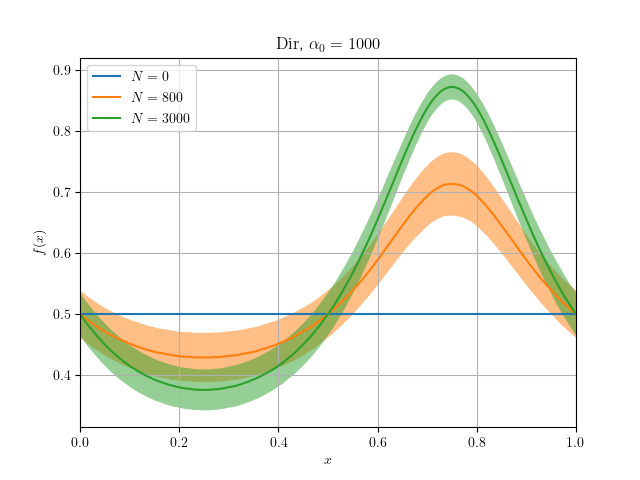
\includegraphics[width=1\linewidth]{Discrete/SE/predict_N.png}
%	\caption{Dirichlet-based predictor mean/variance, varying $N$}
	\label{fig:Discrete/SE/predict_N}
\end{figure}

\end{column}

\end{columns}

\vspace{-1em}
\begin{itemize}
\item Lines show bias $\Erm_{\uppsi | \uptheta}\big[\mu_{\yrm | \xrm, \uppsi}\big]$, fill regions shows variance $\Crm_{\uppsi | \uptheta}\big[\mu_{\yrm | \xrm, \uppsi}\big]$
\item Python simulation results average 50,000 learning iterations
\end{itemize}

\end{frame}




\begin{frame}
\frametitle{Optimal Localization}

\begin{columns}[c]

\begin{column}{.5\linewidth}

For a given conditional mean $\alphac$, localization $\bar{\alpha}_0(x) \equiv \alpha_0 \alpham(x)$ controls a \alert{Bias-Variance} trade-off:
\vspace{-1em}
\begin{table}
\renewcommand{\arraystretch}{1.8}
\scalebox{0.9}{
\begin{tabular}{| c | c | c |}
\hline 
$\bar{\alpha}_0(x)$ & $\lambda_{\text{Bias}}(x; \upthetam)$ & $\lambda_{\text{Var}}(x; \upthetam)$ \\
\hhline{|=|=|=|}
$\to \infty$ & $1$ & $0$ \\
\hline
$\to 0$ & $\big( 1 - \upthetam(x) \big)^N$ & $\Erm_{\uppsim | \upthetam}\left[ \big( N \uppsim(x) \big)^{-1} \right]$  \\ 
\hline
\end{tabular}
}
%\caption{}
\end{table}

\vspace{.5em}
\textbf{Optimal}: 
\vspace{-.5em}
\begin{equation*} \label{eq:alpha_x_min_Rex}
	\bar{\alpha}_0(\xrm) = \frac{\Sigma_{\yrm | \xrm,\upthetac}}{\left( \mu_{\yrm | \xrm} - \mu_{\yrm | \xrm,\upthetac} \right)^2}
\end{equation*}

\end{column}

\begin{column}{.5\linewidth}

\begin{figure}
	\centering
	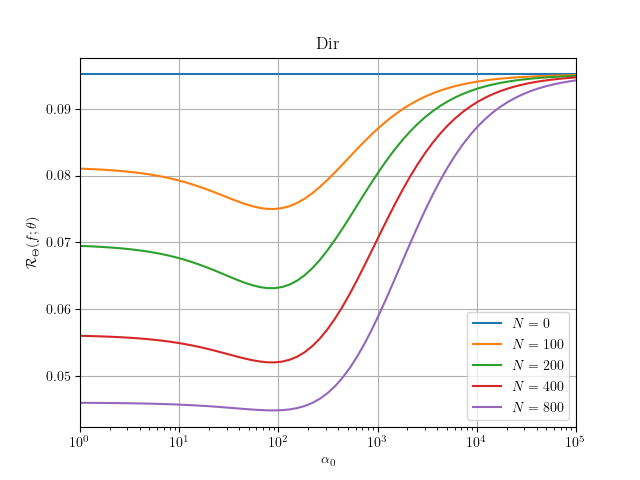
\includegraphics[width=1\linewidth]{Discrete/SE/risk_a0_leg_N.png}
%	\caption{Squared-Error vs. prior localization $\alpha_0$}
	\label{fig:Discrete/SE/risk_a0_leg_N}
\end{figure} 

\end{column}

\end{columns}

\end{frame}




\begin{frame}
\frametitle{Training Volume Trends}

\begin{columns}[c]

\begin{column}{.5\linewidth}

\begin{itemize}
\item As $N \to \infty$, both $\lambda_{\text{Bias}}(\xrm; \upthetam) \to 0$ and $\lambda_{\text{Var}}(\xrm; \upthetam) \to 0$
\begin{itemize}
\item[$\Rightarrow$] $\Rcal_{\Theta, \mathrm{ex}}(f^* ; \uptheta) \to 0$ for \alert{any} model $\uptheta$ 
\end{itemize} 
\vspace{.5em}
\item Note that $f^*(\xrm;\uppsi)$ converges to the clairvoyant regressor \alert{regardless} of how biased the prior conditional mean $\alphac$ is, or how much confidence in $\alphac$ is indicated through the localization $\alpha_0$
\end{itemize}


\end{column}

\begin{column}{.5\linewidth}

\begin{figure}
	\centering
	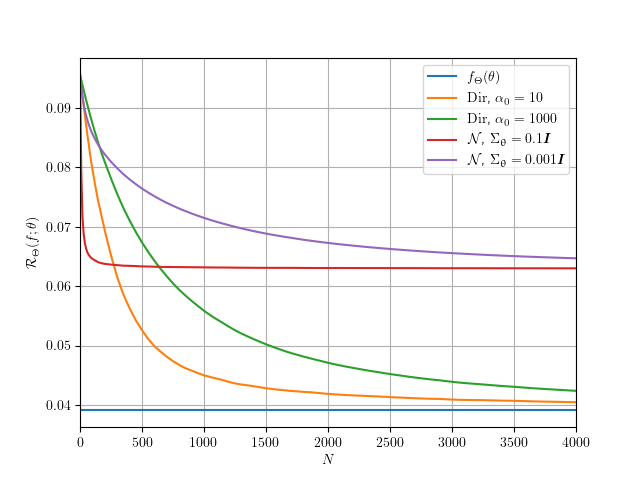
\includegraphics[width=1\linewidth]{Discrete/SE/risk_N_leg_a0.png}
%	\caption{Squared-Error vs. training data volume $N$}
	\label{fig:Discrete/SE/risk_N_leg_a0}
\end{figure}

\end{column}

\end{columns}

\end{frame}





\begin{frame}
\frametitle{Conclusions}

\textbf{Summary}

Full-support Bayesian learning with a Dirichlet prior enables:
\begin{itemize}
\item Asymptotically \alert{optimal} performance for data-rich applications 
\item \alert{Maximal} prior knowledge required for data-limited applications
\end{itemize}

\vspace{1em}
\textbf{Future Work}
\begin{itemize}
\item Generalize these concepts for more general data models using the continuous Dirichlet process \footfullcite{gershman}
\begin{itemize}
\item Practical necessity motivates the use of \alert{discretization} to realize the demonstrated benefits
\end{itemize}
\item Use the Dirichlet prior with different likelihood functions (e.g., mixture model) to effect limited-support priors that may be best suited for data-limited applications
\end{itemize}


\end{frame}







\end{document}
